\begin{figure}[h!]
    \centering
    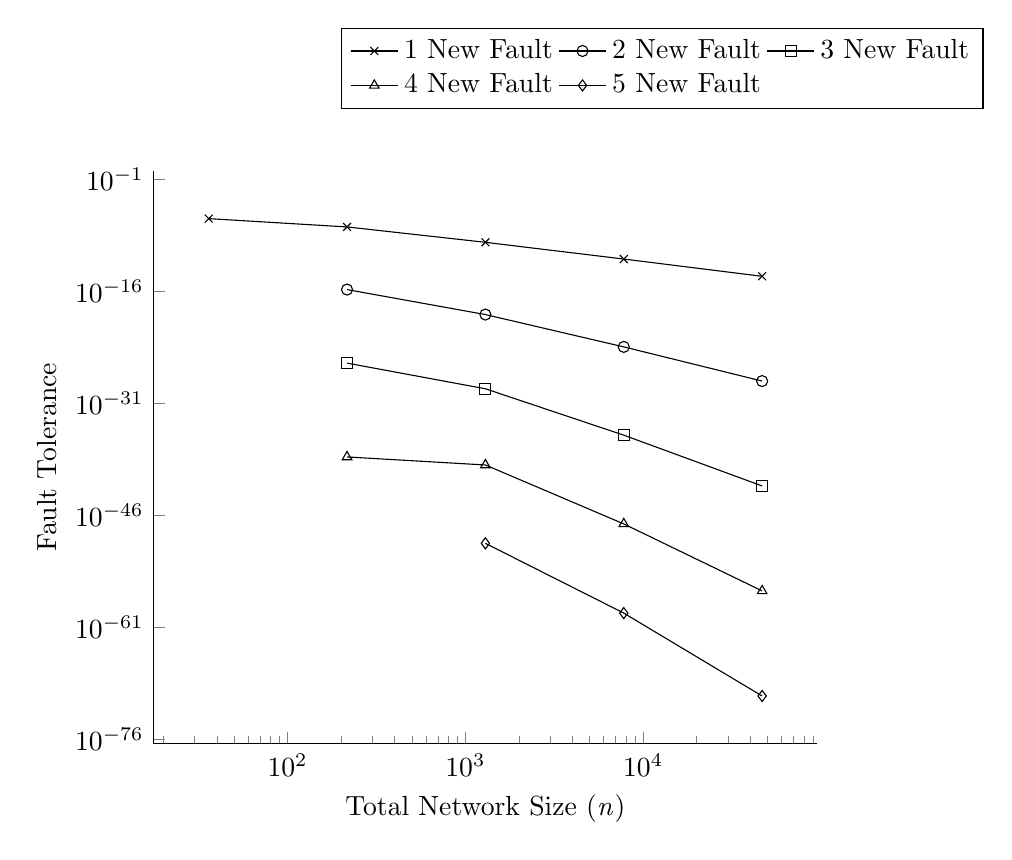
\begin{tikzpicture}
      \pgfplotsset{
          scale only axis,
          every axis legend/.append style={ at={(1.25,1.25)}, 
          legend columns = 3}
      }
    
      \begin{axis}[
        xmode=log,
        ymode=log,
        axis y line*=left,
        axis x line*=bottom,
        xlabel = Total Network Size (\textit{n}),
        ylabel= Fault Tolerance,   
        scaled y ticks=true
      ]

        \addplot[mark=x,color=black] coordinates{
            (36,0.000000513)	
            (216,0.0000000395)	
            (1296, 0.000000000345)	
            (7776,0.00000000000199)	
            (46656,0.00000000000000969)	
            % more points
          }; \label{plot_1_y1}
    
        \addplot[mark=o,color=black] coordinates{
            (216,0.000000000000000162)	
            (1296,0.000000000000000000073)	
            (7776,0.00000000000000000000000344)	
            (46656,0.0000000000000000000000000000908)	
            % more points
          }; \label{plot_1_y2}
          
        \addplot[mark=square,color=black] coordinates{
            (216,0.0000000000000000000000000231)	
            (1296,0.00000000000000000000000000000845)	
            (7776,0.0000000000000000000000000000000000052)	
            (46656,0.000000000000000000000000000000000000000000823)	
            % more points
          }; \label{plot_1_y3}
        
        \addplot[mark=triangle,color=black] coordinates{
            (216,0.0000000000000000000000000000000000000063)	
            (1296,0.000000000000000000000000000000000000000527)	
            (7776,0.00000000000000000000000000000000000000000000000682)	
            (46656,0.00000000000000000000000000000000000000000000000000000000722)	
            % more points
          }; \label{plot_1_y4}
        
        \addplot[mark=diamond,color=black] coordinates{
            (1296,0.000000000000000000000000000000000000000000000000017)	
            (7776,0.00000000000000000000000000000000000000000000000000000000000776)	
            (46656,0.0000000000000000000000000000000000000000000000000000000000000000000000613)	
            % more points
          }; \label{plot_1_y5}
          \addlegendimage{/pgfplots/refstyle=plot_1_y1}\addlegendentry{1 New Fault}
        \addlegendimage{/pgfplots/refstyle=plot_1_y2}\addlegendentry{2 New Fault}
        \addlegendimage{/pgfplots/refstyle=plot_1_y3}\addlegendentry{3 New Fault}
        \addlegendimage{/pgfplots/refstyle=plot_1_y4}\addlegendentry{4 New Fault}

        \addlegendimage{/pgfplots/refstyle=plot_1_y4}\addlegendentry{5 New Fault}
        \end{axis}
    \end{tikzpicture}
    \caption{The likelihood that a new node would become faulty due to \textit{failure bleed} given \(f = \frac{n}{6}\) faulty nodes.}
    \label{fig:failure_f6}
\end{figure}